\setchapterimage[6cm]{chapter/ship/ship_title_image.jpeg}
\setchapterpreamble[u]{\margintoc}
\chapter{Warships and their operators\protect\footnotemark}
\labch{ship}

\footnotetext{Imperial Japanese Navy battleship Fusō prepares for a review at Yokohama, Japan. \href{https://commons.wikimedia.org/wiki/File:Fuso_Yokohama.jpg}{WikiCommons / 1928 / Public domain}. Kure Maritime Museum, (edited by Kazushige Todaka), Japanese Naval Warship Photo Album: Battleships and Battle Cruisers, p. 129.}


This chapter focuses on ships in Russia and in the world. Ships have different purposes, for example: military, civil. Civilian ships are used in a variety of tasks: trucking, fishing, tourism, mineral exploration, rescue work, as well as sports, cultural and other activities. To store a large amount of information about all ships, it is necessary to maintain knowledge bases. One of those knowledge bases is Wikidata. This work is aimed at studying the stored in Wikidata objects describing ships and at evaluating the quality and completeness of their properties and descriptions.


\begin{marginfigure}[0.0cm]
  {
    \setlength{\fboxsep}{0pt}%
    \setlength{\fboxrule}{1pt}%
    \fcolorbox{gray}{gray}{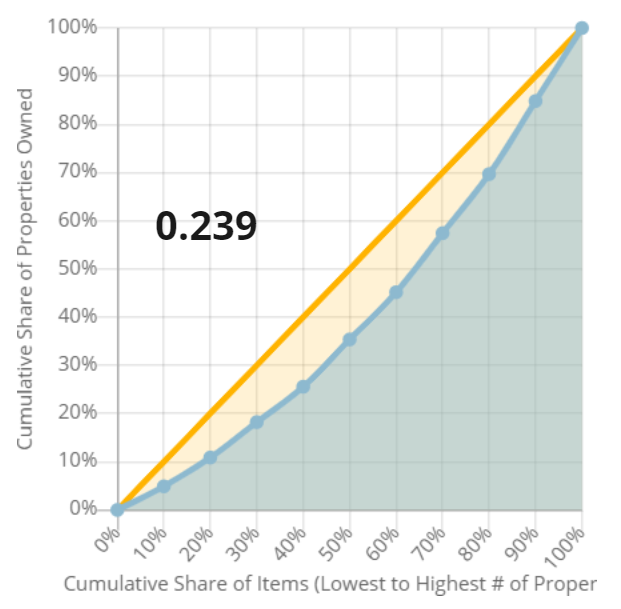
\includegraphics[width=0.9\linewidth]{chapter/ship/Russian_ships_topic_imbalance.png}}
  }
  \caption[Graph of Wikidata objects' completeness]{Graph of \href{https://www.wikidata.org/wiki/Q11446}{ship (Q11446)} Wikidata objects' completeness. Gini coefficient equals 0.239. Data was collected with ProWD.id, 2020. Completeness is not uniform.}%
  \label{fig:prowd_ships-unbalanced}%
\end{marginfigure}

\section{List of ships}

\href{https://en.wikipedia.org/wiki/Ship}{A ship} is a large marine vessel.



Wikidata properties considered in the chapter: 
\begin{itemize}
  \item \href{https://www.wikidata.org/wiki/Property:P31}{instance of (P31)}.
  \item \href{https://www.wikidata.org/wiki/Property:P137}{operator (P137)}.
  \item \href{https://www.wikidata.org/wiki/Property:P17}{country (P17)}.
  \item \href{https://www.wikidata.org/wiki/Property:P607}{conflict (P607)}
\end{itemize}

Let's build a list of all ships with the script in listing \ref{lst:list_of_ship_en}


\begin{lstlisting}[ language=SPARQL, caption={List of ships. \num{19820} ships (2017), \num{50681} ships (2020), \num{71203} ships (2021). SPARQL-query: \href{https://w.wiki/vhp}{https://w.wiki/vhp}}, label=lst:list_of_ship_en, texcl]
# List of ships
SELECT ?ship ?shipLabel
WHERE
{
  ?ship wdt:P31 wd:Q11446. # instance of ship
SERVICE wikibase:label {bd:serviceParam wikibase:language "en"}
}
\end{lstlisting}


\begin{marginfigure}[0.0cm]
  {
    \setlength{\fboxsep}{0pt}%
    \setlength{\fboxrule}{1pt}%
    \fcolorbox{gray}{gray}{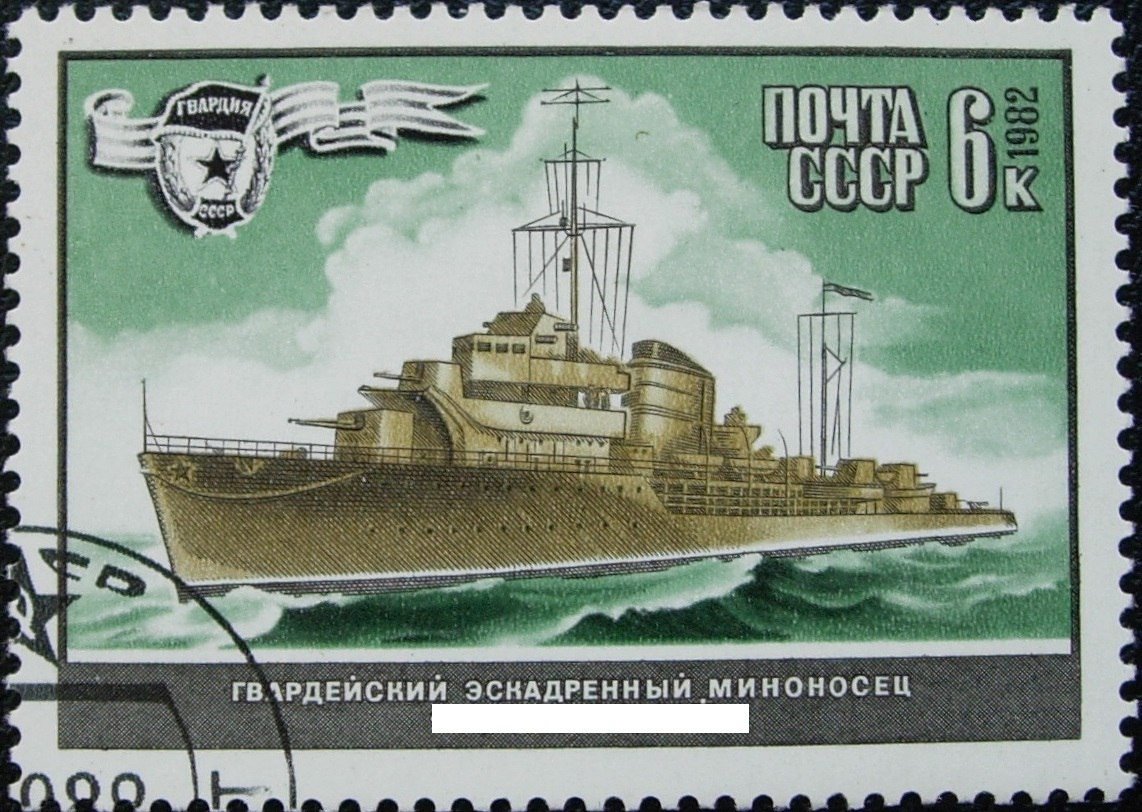
\includegraphics[width=0.95\linewidth]{chapter/ship/Secret_Grem_ship.jpg}}
  }
  \caption[Soviet destroyer project 7]{Postage stamp with a picture of Famous Soviet destroyer project 7.}%
  \label{fig:quiz_question_ship}%
\end{marginfigure}
\label{question:ship_1}
  
\begin{lstlisting}[ language=SPARQL, caption={List of ship from Russia, Soviet Union and Russian Empire. \num{107} ships (2017), \num{579} ships (2020), \num{578} ships (2020). SPARQL-query: \href{https://w.wiki/vhw}{https://w.wiki/vhw}}, label=lst:list_of_ship_ussr_rf_re_en, texcl]
# List of ship from Russia, Soviet Union and Russian Empire
SELECT ?ship ?shipLabel
WHERE
{
  ?ship wdt:P31 wd:Q11446; # instance of ship
        wdt:P137/wdt:P17 ?country.   # belongs to country
    
  VALUES ?country {wd:Q34266 # Russian EMpire
                  wd:Q15180 # Soviet Union
                  wd:Q159}  # Russia
  SERVICE wikibase:label { bd:serviceParam wikibase:language "en" }
}
\end{lstlisting}

The ship \href{https://www.wikidata.org/wiki/Q281147}{Krasin (Q281147)} has the greatest quantity of properties (29) according to ProWD report \sidecite{ProWD_ru_ships}. The ships \href{https://www.wikidata.org/wiki/Q99198666}{Liven (Q99198666)} (5 properties) and \href{https://www.wikidata.org/wiki/Q28155282}{Dispatch (Q28155282)} (4 properties) have the lowest quantity of properties.


\section{Completeness of the Wikidata}

Finding the exact number of ships in the world is a difficult task. After all, data about some of them are top secret, some are private vessels and there is no information about them either. Suppose that the total number of ships is about \num{1600000}, as indicated in the vessel database \sidecite{FleetMon}. The script in the listing \ref{lst:list_of_ship_en} showed only \num{71203} records, which makes up only 4,3\% of the total number of ships. 

As for the Russian ships, the actual civil and military fleets includes \num{17657} ships \sidecite{RussianShips}. At the time when the script in the listing \ref{lst:list_of_ship_ussr_rf_re_en} showed only 579 records, which is only 0.03\% of the total number of Russian ships. 

In the first and in the second case, the difference between the actual number of ships and the result of requests is huge, which indicates the incompleteness of the Wikidata. It is also showed by Fig. \ref{fig:prowd_ships-unbalanced}.


\section{Ships objects' properties completeness}

It is required to find objects of ships that participated in any military conflicts. Let's do this with the scipt in listing \ref{lst:ships_in_conflict_en}.


\begin{lstlisting}[ language=SPARQL, caption={List of ships with countries and war conflicts in English. \num{1400} ships (2017), \num{3586} ships (2020), \num{3567} ships (2020). SPARQL-query: \href{https://w.wiki/vi2}{https://w.wiki/vi2}}, label=lst:ships_in_conflict_en, texcl]
# List of ships with countries and war conflicts
SELECT ?ship ?shipLabel ?countryLabel ?conflict ?conflictLabel
WHERE
{
  ?ship wdt:P31 wd:Q11446;        # instance of ship
        wdt:P137/wdt:P17 ?country;# belongs to country
        wdt:P607 ?conflict.       # engaged in some conflict
SERVICE wikibase:label {bd:serviceParam wikibase:language "en"}
}
\end{lstlisting}

\marginnote{The figure \ref{fig:quiz_question_ship} shows the most famous Soviet \href{https://en.wikipedia.org/wiki/Destroyer}{destroyer} \href{https://en.wikipedia.org/wiki/Gnevny-class_destroyer}{project 7}, awarded the title of "Guards", name it. See answer on page~\pageref{answer:ship_1}.}

With the serarator ";" in the script in the listing \ref{lst:ships_in_conflict_en} it is possible to extract multiple properties of the same object in one line of code. It this script to properties were extracted: \href{https://www.wikidata.org/wiki/Property:P17}{country (P17)} of the \href{https://www.wikidata.org/wiki/Property:P137}{operator (P137)} and \href{https://www.wikidata.org/wiki/Property:P607}{conflict (P607)} Military conflicts and military operations, which are part of wars, are different concepts. Filled data on ships can be roughly divided into two types:

\begin{itemize}
  \item \textbf{Objects in which military operations are combined with military conflicts}. For example, in \href{https://www.wikidata.org/wiki/Q4148613}{Soviet destroyer Gremyashchiy} nine wars / battles, see listing \ref{lst:grem_wars}. Such a large number is due to the fact that the ship took part in many \href{https://en.wikipedia.org/wiki/Arctic_convoys_of_World_War_II}{arctic convoys} which are military operations.

\label{question:ship_2}
\marginnote{Find the "Guinness ship". Choose from: the largest, the longest, the most capacious, etc. See answer on page~\pageref{answer:ship_2}.}

  \item \textbf{Objects in which military operations are separated from military conflicts}. For example, in the British cruiser \href{https://en.wikipedia.org/wiki/HMS_Trinidad_(1940)}{HMS Trinidad} participation in the military campaign and the Arctic convoy are listed as part of World War II with the qualifier \href{https://www.wikidata.org/wiki/Property:P1012}{including (P1012)}. Thus, in the Wikidata, this cruiser has one war/battle.
\end{itemize}


\begin{lstlisting}[ language=SPARQL, caption={War conflicts with \href{https://www.wikidata.org/wiki/Q4148613}{destroyer Gremyashchiy}. \num{10} conflicts are found, 2021. SPARQL-query: \href{https://w.wiki/vi3}{https://w.wiki/vi3}}, label=lst:grem_wars, ]
SELECT ?conflict ?conflictLabel
WHERE
{
  ?ship wdt:P31 wd:Q11446;
        wdt:P607 ?conflict.
      
  FILTER (?ship IN (wd:Q4148613))
                
SERVICE wikibase:label {bd:serviceParam wikibase:language "en"}
}
\end{lstlisting}


For the first type of filling in the scripts with the search for \href{https://www.wikidata.org/wiki/Property:P607}{conflict (P607)} properties, the ships will display more wars/battles than the second. But in this case, the operation \href{https://en.wikipedia.org/wiki/Siege_of_Odessa_(1941)}{The Odessa Defense} will stand alongside \href{https://en.wikipedia.org/wiki/World_War_II}{World War II}, although it is part of this war. In this situation, the output data will not be accurate.

\label{question:ship_3}
\marginnote{Output pictures of those ships, about which the film were shot. If there are no such, then those ships, about which the books were written. See answer on page~\pageref{answer:ship_3}.}

For the second type of filling, scripts in listing \ref{lst:ships_in_conflict_2_en} will clearly distinguish where the war is, and where the military operation, also the data displayed on the chart will be more accurate.

\begin{lstlisting}[ language=SPARQL, caption={List of ship with countries and war conflicts in English. \num{105} ships (2017), \num{86} ships (2020), \num{82} ships (2021). SPARQL-query: \href{https://w.wiki/vhs}{https://w.wiki/vhs}}, label=lst:ships_in_conflict_2_en, texcl]
# List of ship with countries and war conflicts
SELECT ?ship ?shipLabel ?countryLabel ?conflict ?conflictLabel
WHERE
{
  ?ship wdt:P31 wd:Q11446;        # instance of ship
        wdt:P137/wdt:P17 ?country;         # belongs to country
        wdt:P607 ?conflict.       # engaged in some conflict
  
  VALUES ?country {wd:Q34266 # Russian EMpire
                   wd:Q15180 # Soviet Union
                   wd:Q159}  # Russia
  SERVICE wikibase:label { bd:serviceParam wikibase:language "en" }
}
\end{lstlisting}

It is important to notice that the ships from script in listing \ref{ships_in_war_ru} are not necessary connected only with Russia, USSR or Soviet Union.
For example, there is ref{https://www.wikidata.org/wiki/Q653477}{Kasato Maru (Q653477)}. It is a japanese ship but it has multiple operators in the list. This list also includes \href{https://www.wikidata.org/wiki/Q3737187}{Dobroflot (Q3737187)}, this operator owned this ship for some time. It means that the same ship may be owned by different operators in different periods. Owners may be changed time to time.

\begin{figure*}[ht]
  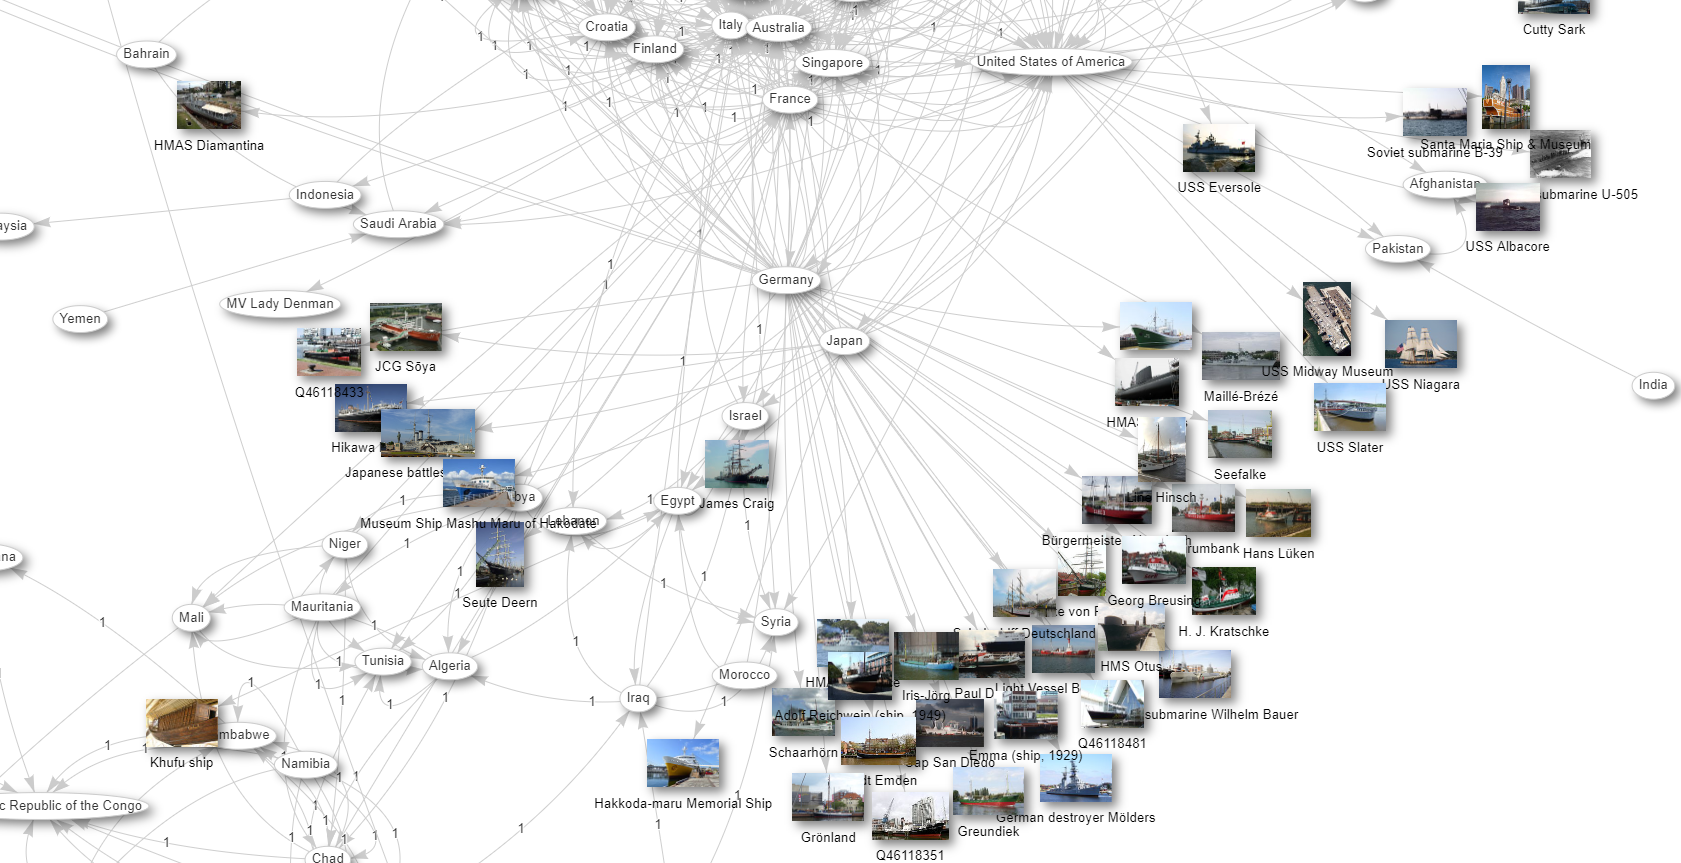
\includegraphics[width=0.9\linewidth]{chapter/ship/museum_graph.png}
  \caption[Graph of countries and museum ships]{Fragment of the graph of countries, museum ships and conflicts, built via the script in the listing \ref{lst:museum_graph}.}%
  \label{fig:museum_graph}%
\end{figure*}
\section{Museum ships around the world}
\href{https://www.wikidata.org/wiki/Q575727}{Museum Ship (Q575727)} -- a ship that houses a museum exhibition dedicated to the history of the ship. Such ships are used for educational and memorial purposes. The ship's participation in the \href{https://www.wikidata.org/wiki/Q180684}{conflict (Q180684)} may lead to the creation of a museum ship in memory of past events.

Let's build a graph of museum ships and the countries in which these ships are located. The vertices of the graph are \href{https://www.wikidata.org/wiki/Q6256}{countries (Q6256)} and \href{https://www.wikidata.org/wiki/Q575727}{museum ships (Q575727)}. The edge between a ship and a country means the ship is in that country. And the edge between the two countries means that there were conflicts between these countries, the number of which is equal to the weight of the edge. The script in listing \ref{lst:museum_graph} builds this graph according to the rules described above.

\begin{lstlisting}[ language=SPARQL, caption={The graph of museum ships and the countries in which these ships are located. 117 vertices are found (2020). SPARQL-query: \href{https://w.wiki/vfj}{https://w.wiki/vfj}}, label=lst:museum_graph, ]
#defaultView:Graph    
SELECT ?vertex1 ?vertex1Label ?vertex2 ?vertex2Label ?edgeLabel ?image 
WHERE {
  {
    # Conflicts
    SELECT ?vertex1 ?vertex1Label ?vertex2 ?vertex2Label 
            (STR(COUNT(?conflict)) as ?edgeLabel) 
    WHERE
    {
      ?conflict wdt:P31 wd:Q180684 .
      ?conflict wdt:P710 ?vertex1, ?vertex2 .
      ?vertex1 wdt:P31 wd:Q6256 . 
      ?vertex2 wdt:P31 wd:Q6256
  
FILTER (?vertex1 != ?vertex2 && STR(?vertex1) < STR(?vertex2))
    
SERVICE wikibase:label {bd:serviceParam wikibase:language "en"}
    }
    GROUP BY ?vertex1 ?vertex1Label ?vertex2 ?vertex2Label
  }
  UNION
  {
    # Museum ships
SELECT DISTINCT ?vertex1 ?vertex1Label ?vertex2 ?vertex2Label ?image
    WHERE
    {
      ?vertex2 wdt:P31 wd:Q575727 .
      {?vertex2 wdt:P17 ?vertex1} UNION # located in country
      {?vertex2 wdt:P131/wdt:P17 ?vertex1}
          
      OPTIONAL { ?vertex2 wdt:P18 ?image}
          
SERVICE wikibase:label {bd:serviceParam wikibase:language "en"}
    }
  }
}
\end{lstlisting}

From a fragment of the graph in figure \ref{fig:museum_graph} it can be seen that the museum ships mostly belong to Germany, the USA and Australia. This "correlation" is quite logical, since these countries have a long history, for which they have participated in many conflicts. Also, these countries have access to the sea, which historically determines the presence of a fleet.

\begin{figure*}[ht]
  {
  \setlength{\fboxsep}{0pt}%
  \setlength{\fboxrule}{1pt}%
  \fcolorbox{gray}{gray}{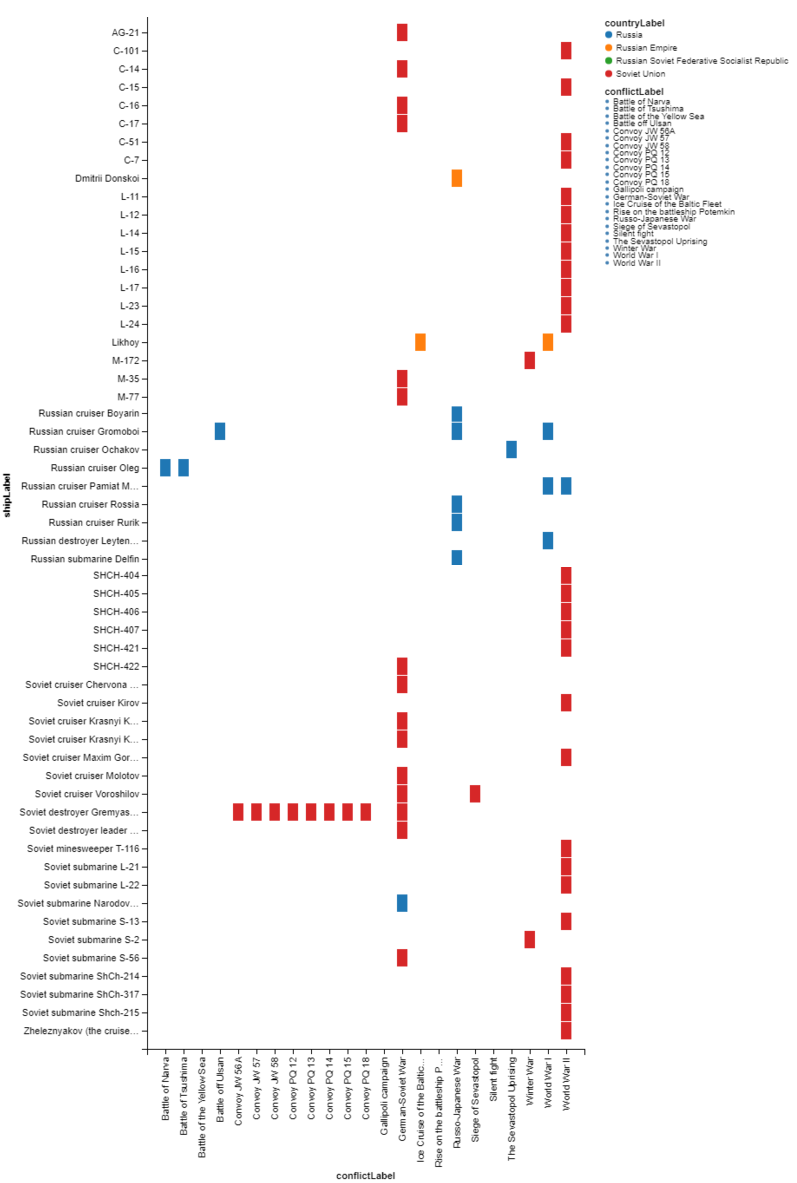
\includegraphics[width=0.95\linewidth]{chapter/ship/List_of_ships_with_countries_and_war_conflicts_in_English.png}}%
  }
    \caption[List of ships with countries and war conflicts]{Fragment of the list of ships with countries and war conflicts (2017). The list shows that most of the ships are associated with Russia and the USSR, as well as with the Second World War or the German-Soviet War.}%
    \label{fig:ships_by_country_and_conflict}%
\end{figure*}